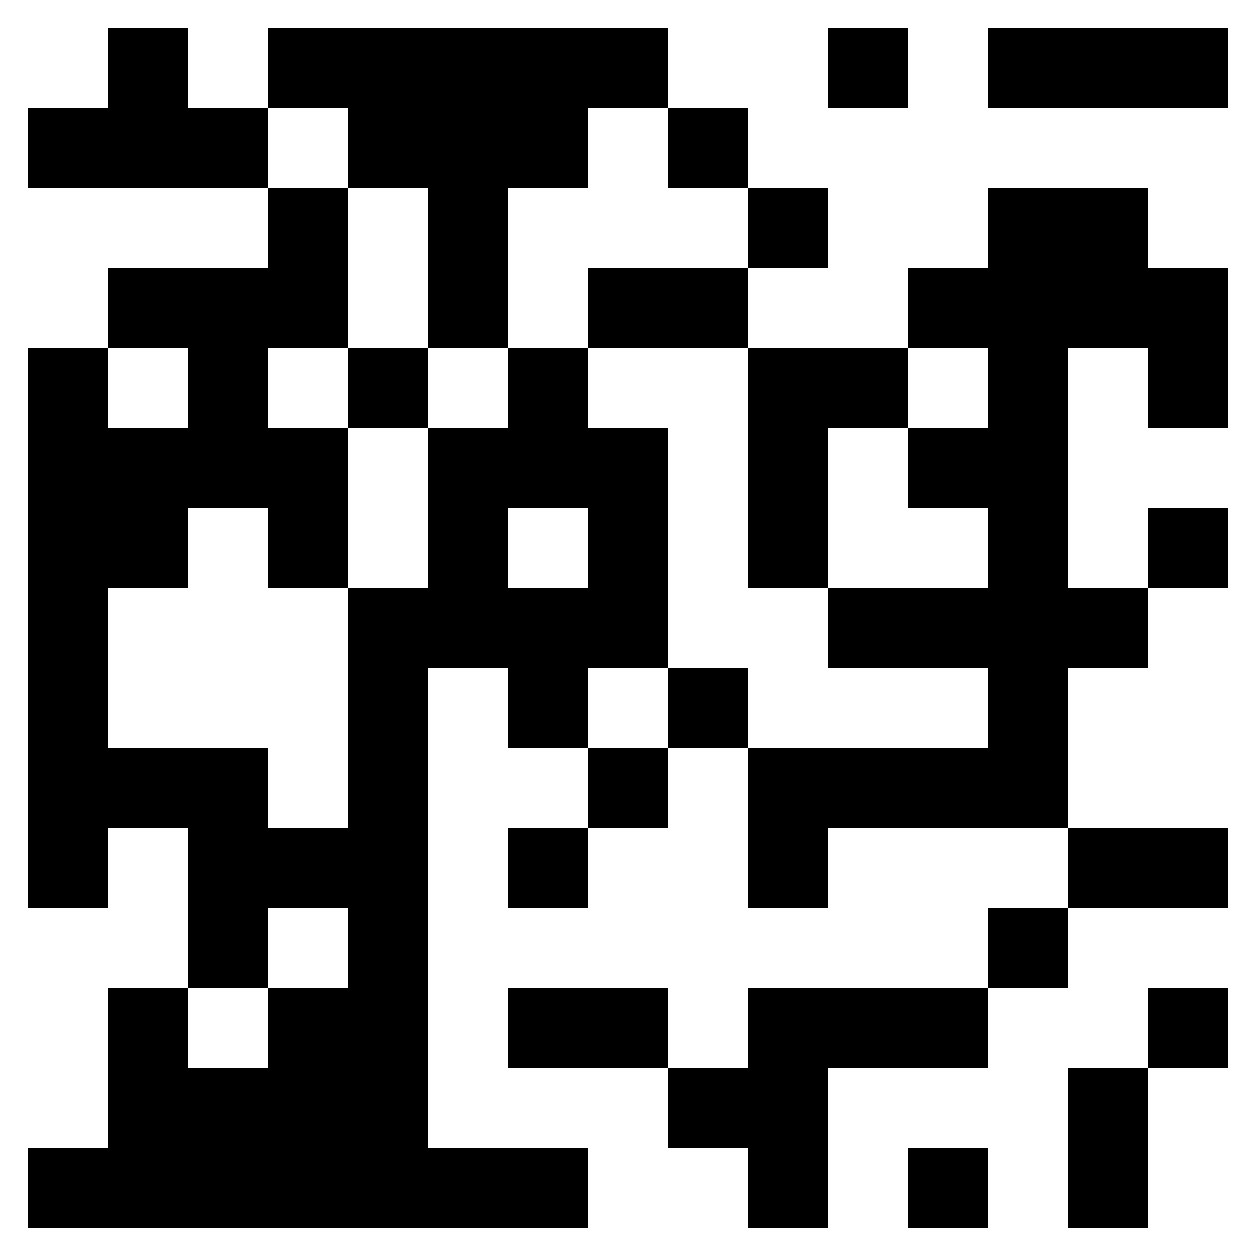
\begin{tikzpicture}[x=0.4in,y=0.4in]
\fill[color=black] (0,0) rectangle (1,1);
\fill[color=white] (0,1) rectangle (1,2);
\fill[color=white] (0,2) rectangle (1,3);
\fill[color=white] (0,3) rectangle (1,4);
\fill[color=black] (0,4) rectangle (1,5);
\fill[color=black] (0,5) rectangle (1,6);
\fill[color=black] (0,6) rectangle (1,7);
\fill[color=black] (0,7) rectangle (1,8);
\fill[color=black] (0,8) rectangle (1,9);
\fill[color=black] (0,9) rectangle (1,10);
\fill[color=black] (0,10) rectangle (1,11);
\fill[color=white] (0,11) rectangle (1,12);
\fill[color=white] (0,12) rectangle (1,13);
\fill[color=black] (0,13) rectangle (1,14);
\fill[color=white] (0,14) rectangle (1,15);
\fill[color=black] (1,0) rectangle (2,1);
\fill[color=black] (1,1) rectangle (2,2);
\fill[color=black] (1,2) rectangle (2,3);
\fill[color=white] (1,3) rectangle (2,4);
\fill[color=white] (1,4) rectangle (2,5);
\fill[color=black] (1,5) rectangle (2,6);
\fill[color=white] (1,6) rectangle (2,7);
\fill[color=black] (1,7) rectangle (2,8);
\fill[color=black] (1,8) rectangle (2,9);
\fill[color=black] (1,9) rectangle (2,10);
\fill[color=white] (1,10) rectangle (2,11);
\fill[color=black] (1,11) rectangle (2,12);
\fill[color=white] (1,12) rectangle (2,13);
\fill[color=black] (1,13) rectangle (2,14);
\fill[color=black] (1,14) rectangle (2,15);
\fill[color=black] (2,0) rectangle (3,1);
\fill[color=black] (2,1) rectangle (3,2);
\fill[color=white] (2,2) rectangle (3,3);
\fill[color=black] (2,3) rectangle (3,4);
\fill[color=black] (2,4) rectangle (3,5);
\fill[color=black] (2,5) rectangle (3,6);
\fill[color=white] (2,6) rectangle (3,7);
\fill[color=black] (2,7) rectangle (3,8);
\fill[color=black] (2,8) rectangle (3,9);
\fill[color=black] (2,9) rectangle (3,10);
\fill[color=black] (2,10) rectangle (3,11);
\fill[color=black] (2,11) rectangle (3,12);
\fill[color=white] (2,12) rectangle (3,13);
\fill[color=black] (2,13) rectangle (3,14);
\fill[color=white] (2,14) rectangle (3,15);
\fill[color=black] (3,0) rectangle (4,1);
\fill[color=black] (3,1) rectangle (4,2);
\fill[color=black] (3,2) rectangle (4,3);
\fill[color=white] (3,3) rectangle (4,4);
\fill[color=black] (3,4) rectangle (4,5);
\fill[color=white] (3,5) rectangle (4,6);
\fill[color=white] (3,6) rectangle (4,7);
\fill[color=white] (3,7) rectangle (4,8);
\fill[color=black] (3,8) rectangle (4,9);
\fill[color=black] (3,9) rectangle (4,10);
\fill[color=white] (3,10) rectangle (4,11);
\fill[color=black] (3,11) rectangle (4,12);
\fill[color=black] (3,12) rectangle (4,13);
\fill[color=white] (3,13) rectangle (4,14);
\fill[color=black] (3,14) rectangle (4,15);
\fill[color=black] (4,0) rectangle (5,1);
\fill[color=black] (4,1) rectangle (5,2);
\fill[color=black] (4,2) rectangle (5,3);
\fill[color=black] (4,3) rectangle (5,4);
\fill[color=black] (4,4) rectangle (5,5);
\fill[color=black] (4,5) rectangle (5,6);
\fill[color=black] (4,6) rectangle (5,7);
\fill[color=black] (4,7) rectangle (5,8);
\fill[color=white] (4,8) rectangle (5,9);
\fill[color=white] (4,9) rectangle (5,10);
\fill[color=black] (4,10) rectangle (5,11);
\fill[color=white] (4,11) rectangle (5,12);
\fill[color=white] (4,12) rectangle (5,13);
\fill[color=black] (4,13) rectangle (5,14);
\fill[color=black] (4,14) rectangle (5,15);
\fill[color=black] (5,0) rectangle (6,1);
\fill[color=white] (5,1) rectangle (6,2);
\fill[color=white] (5,2) rectangle (6,3);
\fill[color=white] (5,3) rectangle (6,4);
\fill[color=white] (5,4) rectangle (6,5);
\fill[color=white] (5,5) rectangle (6,6);
\fill[color=white] (5,6) rectangle (6,7);
\fill[color=black] (5,7) rectangle (6,8);
\fill[color=white] (5,8) rectangle (6,9);
\fill[color=black] (5,9) rectangle (6,10);
\fill[color=white] (5,10) rectangle (6,11);
\fill[color=black] (5,11) rectangle (6,12);
\fill[color=black] (5,12) rectangle (6,13);
\fill[color=black] (5,13) rectangle (6,14);
\fill[color=black] (5,14) rectangle (6,15);
\fill[color=black] (6,0) rectangle (7,1);
\fill[color=white] (6,1) rectangle (7,2);
\fill[color=black] (6,2) rectangle (7,3);
\fill[color=white] (6,3) rectangle (7,4);
\fill[color=black] (6,4) rectangle (7,5);
\fill[color=black] (6,5) rectangle (7,6);
\fill[color=black] (6,6) rectangle (7,7);
\fill[color=black] (6,7) rectangle (7,8);
\fill[color=white] (6,8) rectangle (7,9);
\fill[color=white] (6,9) rectangle (7,10);
\fill[color=black] (6,10) rectangle (7,11);
\fill[color=white] (6,11) rectangle (7,12);
\fill[color=white] (6,12) rectangle (7,13);
\fill[color=black] (6,13) rectangle (7,14);
\fill[color=black] (6,14) rectangle (7,15);
\fill[color=white] (7,0) rectangle (8,1);
\fill[color=white] (7,1) rectangle (8,2);
\fill[color=black] (7,2) rectangle (8,3);
\fill[color=white] (7,3) rectangle (8,4);
\fill[color=black] (7,4) rectangle (8,5);
\fill[color=black] (7,5) rectangle (8,6);
\fill[color=white] (7,6) rectangle (8,7);
\fill[color=black] (7,7) rectangle (8,8);
\fill[color=black] (7,8) rectangle (8,9);
\fill[color=black] (7,9) rectangle (8,10);
\fill[color=white] (7,10) rectangle (8,11);
\fill[color=black] (7,11) rectangle (8,12);
\fill[color=white] (7,12) rectangle (8,13);
\fill[color=white] (7,13) rectangle (8,14);
\fill[color=black] (7,14) rectangle (8,15);
\fill[color=black] (8,0) rectangle (9,1);
\fill[color=black] (8,1) rectangle (9,2);
\fill[color=white] (8,2) rectangle (9,3);
\fill[color=white] (8,3) rectangle (9,4);
\fill[color=white] (8,4) rectangle (9,5);
\fill[color=black] (8,5) rectangle (9,6);
\fill[color=black] (8,6) rectangle (9,7);
\fill[color=white] (8,7) rectangle (9,8);
\fill[color=white] (8,8) rectangle (9,9);
\fill[color=white] (8,9) rectangle (9,10);
\fill[color=white] (8,10) rectangle (9,11);
\fill[color=black] (8,11) rectangle (9,12);
\fill[color=white] (8,12) rectangle (9,13);
\fill[color=black] (8,13) rectangle (9,14);
\fill[color=white] (8,14) rectangle (9,15);
\fill[color=black] (9,0) rectangle (10,1);
\fill[color=black] (9,1) rectangle (10,2);
\fill[color=black] (9,2) rectangle (10,3);
\fill[color=white] (9,3) rectangle (10,4);
\fill[color=black] (9,4) rectangle (10,5);
\fill[color=black] (9,5) rectangle (10,6);
\fill[color=white] (9,6) rectangle (10,7);
\fill[color=white] (9,7) rectangle (10,8);
\fill[color=black] (9,8) rectangle (10,9);
\fill[color=black] (9,9) rectangle (10,10);
\fill[color=black] (9,10) rectangle (10,11);
\fill[color=white] (9,11) rectangle (10,12);
\fill[color=black] (9,12) rectangle (10,13);
\fill[color=white] (9,13) rectangle (10,14);
\fill[color=white] (9,14) rectangle (10,15);
\fill[color=white] (10,0) rectangle (11,1);
\fill[color=white] (10,1) rectangle (11,2);
\fill[color=black] (10,2) rectangle (11,3);
\fill[color=white] (10,3) rectangle (11,4);
\fill[color=white] (10,4) rectangle (11,5);
\fill[color=black] (10,5) rectangle (11,6);
\fill[color=white] (10,6) rectangle (11,7);
\fill[color=black] (10,7) rectangle (11,8);
\fill[color=white] (10,8) rectangle (11,9);
\fill[color=white] (10,9) rectangle (11,10);
\fill[color=black] (10,10) rectangle (11,11);
\fill[color=white] (10,11) rectangle (11,12);
\fill[color=white] (10,12) rectangle (11,13);
\fill[color=white] (10,13) rectangle (11,14);
\fill[color=black] (10,14) rectangle (11,15);
\fill[color=black] (11,0) rectangle (12,1);
\fill[color=white] (11,1) rectangle (12,2);
\fill[color=black] (11,2) rectangle (12,3);
\fill[color=white] (11,3) rectangle (12,4);
\fill[color=white] (11,4) rectangle (12,5);
\fill[color=black] (11,5) rectangle (12,6);
\fill[color=white] (11,6) rectangle (12,7);
\fill[color=black] (11,7) rectangle (12,8);
\fill[color=white] (11,8) rectangle (12,9);
\fill[color=black] (11,9) rectangle (12,10);
\fill[color=white] (11,10) rectangle (12,11);
\fill[color=black] (11,11) rectangle (12,12);
\fill[color=black] (11,12) rectangle (12,13);
\fill[color=white] (11,13) rectangle (12,14);
\fill[color=white] (11,14) rectangle (12,15);
\fill[color=white] (12,0) rectangle (13,1);
\fill[color=white] (12,1) rectangle (13,2);
\fill[color=white] (12,2) rectangle (13,3);
\fill[color=black] (12,3) rectangle (13,4);
\fill[color=white] (12,4) rectangle (13,5);
\fill[color=black] (12,5) rectangle (13,6);
\fill[color=black] (12,6) rectangle (13,7);
\fill[color=black] (12,7) rectangle (13,8);
\fill[color=black] (12,8) rectangle (13,9);
\fill[color=black] (12,9) rectangle (13,10);
\fill[color=black] (12,10) rectangle (13,11);
\fill[color=black] (12,11) rectangle (13,12);
\fill[color=black] (12,12) rectangle (13,13);
\fill[color=white] (12,13) rectangle (13,14);
\fill[color=black] (12,14) rectangle (13,15);
\fill[color=black] (13,0) rectangle (14,1);
\fill[color=black] (13,1) rectangle (14,2);
\fill[color=white] (13,2) rectangle (14,3);
\fill[color=white] (13,3) rectangle (14,4);
\fill[color=black] (13,4) rectangle (14,5);
\fill[color=white] (13,5) rectangle (14,6);
\fill[color=white] (13,6) rectangle (14,7);
\fill[color=black] (13,7) rectangle (14,8);
\fill[color=white] (13,8) rectangle (14,9);
\fill[color=white] (13,9) rectangle (14,10);
\fill[color=white] (13,10) rectangle (14,11);
\fill[color=black] (13,11) rectangle (14,12);
\fill[color=black] (13,12) rectangle (14,13);
\fill[color=white] (13,13) rectangle (14,14);
\fill[color=black] (13,14) rectangle (14,15);
\fill[color=white] (14,0) rectangle (15,1);
\fill[color=white] (14,1) rectangle (15,2);
\fill[color=black] (14,2) rectangle (15,3);
\fill[color=white] (14,3) rectangle (15,4);
\fill[color=black] (14,4) rectangle (15,5);
\fill[color=white] (14,5) rectangle (15,6);
\fill[color=white] (14,6) rectangle (15,7);
\fill[color=white] (14,7) rectangle (15,8);
\fill[color=black] (14,8) rectangle (15,9);
\fill[color=white] (14,9) rectangle (15,10);
\fill[color=black] (14,10) rectangle (15,11);
\fill[color=black] (14,11) rectangle (15,12);
\fill[color=white] (14,12) rectangle (15,13);
\fill[color=white] (14,13) rectangle (15,14);
\fill[color=black] (14,14) rectangle (15,15);

\begin{scope}[shift={(5,8)}] %T
  \fill[color=white] (0,0) rectangle (2,3);
%  \draw[color=cyan,thick] (0,0) rectangle (2,3);
  \fill[color=white] (0,2) rectangle (1,3);
  \fill[color=black] (1,2) rectangle (2,3);
  \fill[color=black] (0,1) rectangle (1,2);
  \fill[color=black] (1,1) rectangle (2,2);
  \fill[color=black] (0,0) rectangle (1,1);
  \fill[color=white] (1,0) rectangle (2,1);
%  \node[transform shape,color=red,anchor=west] at (2,1.5) {$\uparrow$};
\end{scope}
\begin{scope}[shift={(10,3)},rotate=180] %R
  \fill[color=white] (0,0) rectangle (2,3);
%  \draw[color=cyan,thick] (0,0) rectangle (2,3);
  \fill[color=black] (0,2) rectangle (1,3);
  \fill[color=white] (1,2) rectangle (2,3);
  \fill[color=black] (0,1) rectangle (1,2);
  \fill[color=black] (1,1) rectangle (2,2);
  \fill[color=black] (0,0) rectangle (1,1);
  \fill[color=white] (1,0) rectangle (2,1);
%  \node[transform shape,color=red,anchor=west] at (2,1.5) {$\uparrow$};
\end{scope}
\begin{scope}[shift={(1,6)}] %A
  \fill[color=white] (0,0) rectangle (2,3);
%  \draw[color=cyan,thick] (0,0) rectangle (2,3);
  \fill[color=black] (0,2) rectangle (1,3);
  \fill[color=white] (1,2) rectangle (2,3);
  \fill[color=white] (0,1) rectangle (1,2);
  \fill[color=white] (1,1) rectangle (2,2);
  \fill[color=white] (0,0) rectangle (1,1);
  \fill[color=white] (1,0) rectangle (2,1);
%  \node[transform shape,color=red,anchor=west] at (2,1.5) {$\uparrow$};
\end{scope}
\begin{scope}[shift={(10,13)},rotate=-90] %D
  \fill[color=white] (0,0) rectangle (2,3);
%  \draw[color=cyan,thick] (0,0) rectangle (2,3);
  \fill[color=black] (0,2) rectangle (1,3);
  \fill[color=black] (1,2) rectangle (2,3);
  \fill[color=white] (0,1) rectangle (1,2);
  \fill[color=black] (1,1) rectangle (2,2);
  \fill[color=white] (0,0) rectangle (1,1);
  \fill[color=white] (1,0) rectangle (2,1);
%  \node[transform shape,color=red,anchor=west] at (2,1.5) {$\uparrow$};
\end{scope}
\begin{scope}[shift={(9,4)},rotate=90] %E
  \fill[color=white] (0,0) rectangle (2,3);
%  \draw[color=cyan,thick] (0,0) rectangle (2,3);
  \fill[color=black] (0,2) rectangle (1,3);
  \fill[color=white] (1,2) rectangle (2,3);
  \fill[color=white] (0,1) rectangle (1,2);
  \fill[color=black] (1,1) rectangle (2,2);
  \fill[color=white] (0,0) rectangle (1,1);
  \fill[color=white] (1,0) rectangle (2,1);
%  \node[transform shape,color=red,anchor=west] at (2,1.5) {$\uparrow$};
\end{scope}
\end{tikzpicture}
\newpage
\begin{tikzpicture}[x=0.4in,y=0.4in,rotate=90]
\fill[color=white] (0,0) rectangle (15,15);
\node at (0,0) {$+$};
\node at (15,0) {$+$};
\begin{scope}[shift={(5,8)}] %T
  \fill[color=white] (0,0) rectangle (2,3);
  \draw[color=black,thick] (0,0) rectangle (2,3);
%  \fill[color=white] (0,2) rectangle (1,3);
%  \fill[color=black] (1,2) rectangle (2,3);
%  \fill[color=black] (0,1) rectangle (1,2);
%  \fill[color=black] (1,1) rectangle (2,2);
%  \fill[color=black] (0,0) rectangle (1,1);
%  \fill[color=white] (1,0) rectangle (2,1);
  \node[transform shape,color=red,anchor=west] at (2,1.5) {$\uparrow$};
  \node[transform shape] at (1,1.5) {1};
\end{scope}
\begin{scope}[shift={(10,3)},rotate=180] %R
  \fill[color=white] (0,0) rectangle (2,3);
  \draw[color=black,thick] (0,0) rectangle (2,3);
%  \fill[color=black] (0,2) rectangle (1,3);
%  \fill[color=white] (1,2) rectangle (2,3);
%  \fill[color=black] (0,1) rectangle (1,2);
%  \fill[color=black] (1,1) rectangle (2,2);
%  \fill[color=black] (0,0) rectangle (1,1);
%  \fill[color=white] (1,0) rectangle (2,1);
  \node[transform shape,color=red,anchor=west] at (2,1.5) {$\uparrow$};
  \node[transform shape] at (1,1.5) {2};
\end{scope}
\begin{scope}[shift={(1,6)}] %A
  \fill[color=white] (0,0) rectangle (2,3);
  \draw[color=black,thick] (0,0) rectangle (2,3);
%  \fill[color=black] (0,2) rectangle (1,3);
%  \fill[color=white] (1,2) rectangle (2,3);
%  \fill[color=white] (0,1) rectangle (1,2);
%  \fill[color=white] (1,1) rectangle (2,2);
%  \fill[color=white] (0,0) rectangle (1,1);
%  \fill[color=white] (1,0) rectangle (2,1);
  \node[transform shape,color=red,anchor=west] at (2,1.5) {$\uparrow$};
  \node[transform shape] at (1,1.5) {3};
\end{scope}
\begin{scope}[shift={(10,13)},rotate=-90] %D
  \fill[color=white] (0,0) rectangle (2,3);
  \draw[color=black,thick] (0,0) rectangle (2,3);
%  \fill[color=black] (0,2) rectangle (1,3);
%  \fill[color=black] (1,2) rectangle (2,3);
%  \fill[color=white] (0,1) rectangle (1,2);
%  \fill[color=black] (1,1) rectangle (2,2);
%  \fill[color=white] (0,0) rectangle (1,1);
%  \fill[color=white] (1,0) rectangle (2,1);
  \node[transform shape,color=red,anchor=west] at (2,1.5) {$\uparrow$};
  \node[transform shape] at (1,1.5) {4};
\end{scope}
\begin{scope}[shift={(9,4)},rotate=90] %E
  \fill[color=white] (0,0) rectangle (2,3);
  \draw[color=black,thick] (0,0) rectangle (2,3);
%  \fill[color=black] (0,2) rectangle (1,3);
%  \fill[color=white] (1,2) rectangle (2,3);
%  \fill[color=white] (0,1) rectangle (1,2);
%  \fill[color=black] (1,1) rectangle (2,2);
%  \fill[color=white] (0,0) rectangle (1,1);
%  \fill[color=white] (1,0) rectangle (2,1);
  \node[transform shape,color=red,anchor=west] at (2,1.5) {$\uparrow$};
  \node[transform shape] at (1,1.5) {5};
\end{scope}
\begin{scope}[shift={(2,1)}]
  \draw[color=black,thick] (0,0) rectangle (2,3);
  \node[transform shape,color=red,anchor=west] at (2,1.5) {$\uparrow$};
\end{scope}
\begin{scope}[shift={(1,12)},rotate=-90]
  \draw[color=black,thick] (0,0) rectangle (2,3);
  \node[transform shape,color=red,anchor=west] at (2,1.5) {$\uparrow$};
\end{scope}
\begin{scope}[shift={(10,10)},rotate=180]
  \draw[color=black,thick] (0,0) rectangle (2,3);
  \node[transform shape,color=red,anchor=west] at (2,1.5) {$\uparrow$};
\end{scope}
\begin{scope}[shift={(14,5)},rotate=90]
  \draw[color=black,thick] (0,0) rectangle (2,3);
  \node[transform shape,color=red,anchor=west] at (2,1.5) {$\uparrow$};
\end{scope}
\end{tikzpicture}

TODOs: Cluekeeper will tell players to put the \(+\)s on the bottom
of the qr code looking thing. And obviously the 1/2/3/4/5 needs to be
replaced with some sort of extraction from the main puzzle.
